\documentclass{sigchi}

% Use this command to override the default ACM copyright statement
% (e.g. for preprints).  Consult the conference website for the
% camera-ready copyright statement.


%% EXAMPLE BEGIN -- HOW TO OVERRIDE THE DEFAULT COPYRIGHT STRIP -- (July 22, 2013 - Paul Baumann)
% \toappear{Permission to make digital or hard copies of all or part of this work for personal or classroom use is      granted without fee provided that copies are not made or distributed for profit or commercial advantage and that copies bear this notice and the full citation on the first page. Copyrights for components of this work owned by others than ACM must be honored. Abstracting with credit is permitted. To copy otherwise, or republish, to post on servers or to redistribute to lists, requires prior specific permission and/or a fee. Request permissions from permissions@acm.org. \\
% {\emph{CHI'14}}, April 26--May 1, 2014, Toronto, Canada. \\
% Copyright \copyright~2014 ACM ISBN/14/04...\$15.00. \\
% DOI string from ACM form confirmation}
%% EXAMPLE END -- HOW TO OVERRIDE THE DEFAULT COPYRIGHT STRIP -- (July 22, 2013 - Paul Baumann)


% Arabic page numbers for submission.  Remove this line to eliminate
% page numbers for the camera ready copy 

%\pagenumbering{arabic}

% Load basic packages
\usepackage{balance}  % to better equalize the last page
\usepackage{graphics} % for EPS, load graphicx instead 
%\usepackage[T1]{fontenc}
\usepackage{txfonts}
\usepackage{times}    % comment if you want LaTeX's default font
\usepackage[pdftex]{hyperref}
% \usepackage{url}      % llt: nicely formatted URLs
\usepackage{color}
\usepackage{textcomp}
\usepackage{booktabs}
\usepackage{ccicons}
\usepackage{todonotes}

% llt: Define a global style for URLs, rather that the default one
\makeatletter
\def\url@leostyle{%
  \@ifundefined{selectfont}{\def\UrlFont{\sf}}{\def\UrlFont{\small\bf\ttfamily}}}
\makeatother
\urlstyle{leo}

% To make various LaTeX processors do the right thing with page size.
\def\pprw{8.5in}
\def\pprh{11in}
\special{papersize=\pprw,\pprh}
\setlength{\paperwidth}{\pprw}
\setlength{\paperheight}{\pprh}
\setlength{\pdfpagewidth}{\pprw}
\setlength{\pdfpageheight}{\pprh}

% Make sure hyperref comes last of your loaded packages, to give it a
% fighting chance of not being over-written, since its job is to
% redefine many LaTeX commands.
\definecolor{linkColor}{RGB}{6,125,233}
\hypersetup{%
  pdftitle={SIGCHI Conference Proceedings Format},
  pdfauthor={LaTeX},
  pdfkeywords={SIGCHI, proceedings, archival format},
  bookmarksnumbered,
  pdfstartview={FitH},
  colorlinks,
  citecolor=black,
  filecolor=black,
  linkcolor=black,
  urlcolor=linkColor,
  breaklinks=true,
}

% create a shortcut to typeset table headings
% \newcommand\tabhead[1]{\small\textbf{#1}}

% End of preamble. Here it comes the document.
\begin{document}

\title{A Conceptual Framework for Evaluating and Designing Information Discovery and Curation Web Tools}

\numberofauthors{3}
\author{%
  \alignauthor{Elena Voyloshnikova\\
    \affaddr{University of Victoria}\\
    \affaddr{Victoria, Canada}\\
    \email{elenavoyl@gmail.com}}\\
  \alignauthor{Margaret-Anne Storey\\
    \affaddr{University of Victoria}\\
    \affaddr{Victoria, Canada}\\
    \email{mstorey@uvic.ca}}\\
}

\maketitle

\begin{abstract}
  UPDATED---\today. Everyday life revolves around the discovery and curation of digital information. People search the Web continuously, from quickly looking up the information needed to complete a task, to endlessly searching for inspiration and knowledge. A variety of studies have modeled information seeking strategies and characterized information seeking and curation activities on the Web. However, there is a lack of research on how existing Web applications support the discovery and curation of information, especially concerning the motivations behind them and how different approaches can be compared. In this paper, we present a study of information discovery tools and how they relate to the nature of information seeking. We propose a conceptual framework that deals with Web application design elements that support different aspects of information discovery and curation. This framework can be used when designing, evaluating or updating Web applications.
\end{abstract}

\keywords{
%Authors' choice; of terms; separated; by semi\-colons; commas, within terms only; this section is required.
  }

\category{H.5.m.}{Information Interfaces and Presentation (e.g. HCI)}{Miscellaneous} \category{See\url{http://acm.org/about/class/1998/} for the full list of ACM classifiers. This section is required.}{}{}

\section{Introduction}

Web technologies help people satisfy their information needs. People research their interests and hobbies using various online resources, shoppers search online stores for product characteristics to make purchasing decisions, and travelers visit online booking sites to find information about flights and hotels. In order to accommodate diverse and evolving user needs, Web applications continuously introduce new features and services, empowering information discovery and curation. 

The term ``information discovery'' has been used by many researchers to define or explain various information behaviour paradigms, such as information exploration~\cite{waterworth1991model} and serendipitous information seeking~\cite{foster2003serendipity}. However, the definition of information discovery itself is difficult to articulate. 

Lynch describes resource discovery as a complex collection of activities ranging from locating a well-specified information to iterative research activities, that can involve the identification
of potentially relevant resources, organization and ranking of resources, and resource exploration~\cite{lynch1995networked}. Proper and Bruza apply the term ``information discovery'' in the context of  the identification and retrieval of relevant information from electronic sources~\cite{proper1999information}. 

In the field of cognitive psychology, Jerome S. Bruner~\cite{bruner1961act} defines information discovery as ``all forms of obtaining knowledge for oneself by the use of one's own mind.'' We build on Bruner's definition to underline the importance of the cognitive processes that govern information discovery. Therefore, we consider \textit{information discovery} as a process of obtaining knowledge from digital sources that can involve complex mental tasks and information behavior.  

Information behavior refers to the totality of ways in which humans interact with information~\cite{wilson2000human}. It can enable and support information discovery when targeted at information maintenance and augmentation. This type of information behavior is also known as \textit{digital curation}.

Similar to the term ``information discovery'', the term "digital curation" is perceived differently across disciplines and among researchers. In this thesis, we use the definition proposed by Giaretta~\cite{giaretta2006dcc} and adopted by the Digital Curation Centre\footnote{The Digital Curation Centre is a UK-based organization established to support expertise and practice in digital curation and preservation across communities of practice.} which states that digital curation is a process of maintaining and adding value to an existing body of information to improve its future use and retrieval.   

Information discovery can take on many forms. Web users might be hoping to find particular pieces of information, such as show times and phone numbers, to satisfy specific information needs~\cite{proper1999information}. Alternatively, they might be lacking well-articulated information needs, so they engage in opportunistic browsing~\cite{lindley2012s}. Sometimes people discover information online without even looking for it~\cite{bates1986exploratory}. The nature of information discovery can vary, and therefore, it requires elaborate tool support. The functionality required for information discovery and curation can also be distributed among multiple applications, which often leads to tools that provide integrated solutions. With people having such diverse information needs and methods of looking for information, designing for information discovery is a challenging task~\cite{conaway2010designing, marchionini2006exploratory}.

Our research goal is to gain an understanding of how existing tools support digital information discovery and curation addressing the problem of designing Web applications for information discovery. While several researchers propose frameworks targeted at designing information discovery systems~\cite{proper1999information, kerne2004information}, the importance of information curation in the realm of information discovery has been largely overlooked despite the rapidly increasing popularity of socially-curated information spaces. Moreover, much of the existing work that focuses on how people look for and discover information online~\cite{bates1986exploratory, choo2000information, ellis1989behavioural, kellar2006goal, lindley2012s, morrison2001taxonomic, sellen2002knowledge} fails to examine concrete features of existing Web-based information discovery applications that empower real-world users. More research is necessary to determine how different tools and their features provide fundamental support for information discovery and curation.

To enhance information seeking and curating experiences and support users' interactions, we extend existing research by (1) deriving factors that enable information discovery and curation and relating them within a framework, (2) using the framework to establish a set of questions that can be used when evaluating and designing new applications, (3) iteratively evaluating the framework by using it to study and describe current Web applications as well as to design a new application, which in turn helped refine the framework of factors and questions, and (4) relating the framework to user information discovery and curation motives that drive the underlying usage of many Web-based applications.

%SAMPLE FIGURES AND TABLES
%\begin{figure}
%\centering
%  
\includegraphics[width=0.9\columnwidth]{figures/sigchi-logo}
% \caption{Insert a caption below each figure. Do not alter the
%    Caption style.}~\label{fig:figure1}
%\end{figure}
%
%\begin{table}
%  \centering
%  \begin{tabular}{r c c}
%    \toprule
%    & \multicolumn{2}{c}{\small{\textbf{Caption}}} \\
%    \cmidrule(r){2-3}
%    {\small\textbf{Objects}}
%    & {\small \textit{Pre-2002}}
%    & {\small \textit{Current}} \\
%    \midrule
%    Tables & Above & Below \\
%    Figures & Below & Below \\
%    \bottomrule
%  \end{tabular}
%  \caption{Table captions should be placed below the table. We
%    recommend table lines be 1 point, 25\% black. Minimize use of
%    unnecessary table lines.}~\label{tab:table1}
%\end{table}
%
%\begin{figure*}
%  \centering
%  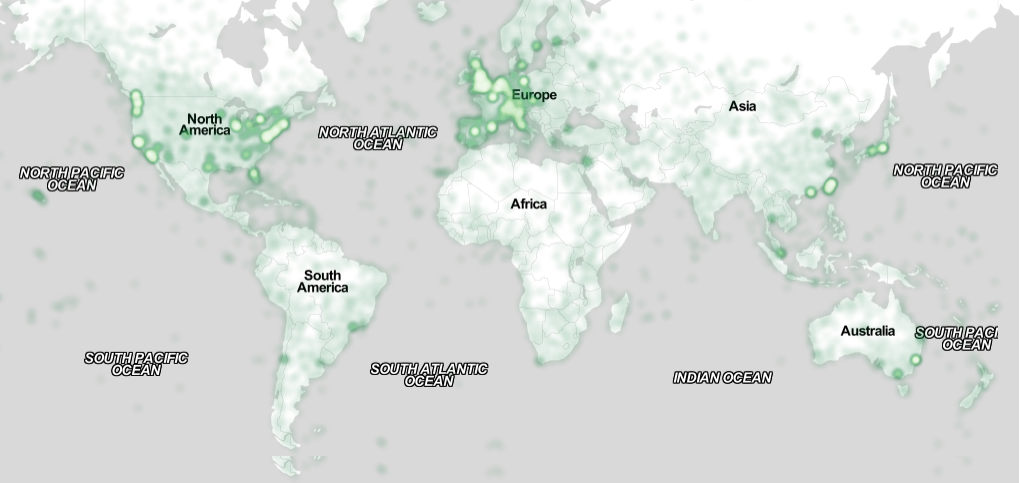
\includegraphics[width=2\columnwidth]{figures/map}
%  \caption{In this image, the map maximizes use of space. You can make
%    figures as wide as you need, up to a maximum of the full width of
%    both columns. Note that \LaTeX\ tends to render large figures on a
%    dedicated page. Image: \ccbynd~ayman on
%    Flickr.}~\label{fig:figure2}
%\end{figure*}
%
%\begin{itemize}
%\item Write in a straightforward style.
%\end{itemize}

\section{Web-based Information Discovery and Curation}
Given the complexity of Web-based information discovery and curation tasks, a variety of research topics are examined to gain an understanding of how current Web tools support these tasks, including information-related Web usage characteristics, current information behavior models, and other aspects of information discovery and curation.  This section outlines the key background literature that contributed to the development of the conceptual framework and helped answer the research questions. 

\subsection{Information Behavior}
Information behavior refers to the totality of ways in which humans behave in relation to information~\cite{wilson2000human}.  A number of models and frameworks have attempted to represent human information behaviour in its entirety or to represent some of its components, such as information seeking and searching, information retrieval, information discovery, and information curation. 

One of the early information behavior models was proposed by Wilson~\cite{wilson1981user} in 1981. It states that information seeking behavior results from the user trying to satisfy a perceived information need, and consequently, the user makes demands on information systems. Success or failure of such demands dictates whether the process is repeated or, if the information need is satisfied, it is used or communicated with other people. 

These underlying ideas remained in the revision of Wilson's model~\cite{wilson1997information} in 1997. In the new model, however, Wilson defined possible barriers (psychological, environments, demographic, etc.) that can impede information seeking. Additionally, the model recognizes that information seeking behaviour can take on many forms and is not limited to active searching. Saracevic~\cite{saracevic1996modeling} and Ingwersen~\cite{ingwersen1996cognitive} derived comparable models that focus on human behaviour when interacting with information retrieval systems. 

\subsubsection{Information Seeking Models}
\textit{Information seeking} refers to ``the purposive seeking for information as a consequence of a need to satisfy some goal~\cite{wilson2000human}.'' A number of researchers have tried to identify what different modes of information seeking behaviour may entail. 

According to Kellar et al.~\cite{kellar2006goal}, information seeking is composed of browsing, fact finding, and information gathering. Although the authors categorized information gathering as part of information seeking, it appears to be more closely related to digital curation~\cite{beagrie2008digital,whittaker2011personal}. 

Bates~\cite{bates1986exploratory,bates2002toward} proposed a model of four information seeking modes: being aware, monitoring, browsing, and searching. Bates differentiated the modes based on the user's level of attention being active or passive, and information needs being directed or undirected. Thus, browsing can be characterized as undirected active information seeking because users do not know exactly what information they are looking for, but they are actively looking. Searching falls under active directed information seeking because the information need is clearly defined and the search is directed. Finally, monitoring and being aware are passive modes of information seeking although monitoring is directed and being aware is undirected.

Ellis et al.~\cite{ellis1989behavioural,ellis1993comparison,ellis1997modelling} proposed a model of information seeking characterized by six different patterns: starting, chaining, browsing, extracting, monitoring, and differentiating. Ellis' model complemented Kuhlthau's work, which correlated stages of information seeking with feelings, thoughts, actions, as well as anticipated information tasks~\cite{kuhlthau1991inside}.

Finally, Wilson also proposed a ``problem solving model'' of information seeking behavior~\cite{wilson1999models}. The model reflects on the idea that people engage in information seeking and searching in order to resolve some uncertainty that stands in the way of solving, defining, or identifying a problem.  

\subsubsection{Information Exploration}
\textit{Information exploration}, or exploratory search, does not have a single definition in the realm of information behavior. Waterworth highlights that exploration is a "broad" activity and identifies browsing as an example of exploration~\cite{waterworth1991model}. According to Marchionini~\cite{marchionini2006exploratory}, exploratory search involves learning (knowledge acquisition, comparison, comprehension, etc.) and investigating (analysis, synthesis, evaluation, discovery, etc.) Similar to Janiszewski ~\cite{janiszewski1998influence}, in terms of information exploration, our focus is on the visual aspects of information exploration, specifically visual and spatial data representations.

\subsubsection{Information Foraging}
\textit{Information foraging theory} is another approach towards understanding how people adapt their strategies of interacting with technology when seeking, gathering, or consuming information, depending on the environment~\cite{pirolli1999information}. The theory resonates with explanations of human behavior in the context of food foraging. 

The underlying assumption of the information foraging theory is that people, similarly to when they forage for food, adopt their foraging strategies to the environment in order to gain the maximum amount of valuable information. The theory states that ``natural information systems evolve towards stable states that maximize gains of valuable information per unit cost.''

The theory introduces three key concepts to formulate an understanding of information foraging: information scent, information diet, and information patch. An \textit{information scent} refers to proximal cues (often visual or linguistic) that people use to identify the value of information. An \textit{information diet} deals with user preferences when it comes to information. At last, \textit{information patches} are clusters of information that an information system presents before the user. The theory with these concepts lays the foundation for existing information foraging models~\cite{fu2007snif,kitajima2000comprehension} as well as social information foraging models~\cite{pirolli2009elementary,fu2008microstructures}.  


\subsubsection{Information Discovery}
Kerne and Smith proposed an information discovery framework~\cite{kerne2004information} that connects human cognitive processes or states to those of an information system. The framework represents a continuum of information flowing through different system and cognitive states as a result of an iterative reformulation process. The framework consists of five mental states: formulating a problem, evaluating results, updating and forming mental models, running mental models, and discovering solutions. Each mental state has a corresponding interaction with the system. For example, browsing resources (human-system interaction) facilitates evaluation or immediate results (cognitive state). The framework helps to understand the user's cognitive processes and provide affordances that facilitate information discovery.
   
\subsubsection{Digital Curation}
In 2002, Bates extended her research on the topic of information behaviour with the notion of \textit{information farming}, which involves people collecting and organizing information for future use and revisitation~\cite{bates2002toward}. More commonly, information farming is referred to as digital curation. 

Wittaker believes that in terms of Web use, a significant shift is happening from information consumption to information curation. People no longer use the Web just to find and consume the information they are interested in, but they also try to save and manage that information so that it can be reaccessed and exploited later~\cite{whittaker2011personal}. 

Existing models and frameworks for information seeking, searching, exploration, discovery, and curation all try to explain human information-related behavior using different but comparable terminology. They help establish an understanding of how humans interact with information. However, many of them either fail to address required tool support for information-related activities or address it at a very high-level.  

\subsection{Web Tasks and Modes of Web Use}
Outside the realm of cognitive models and frameworks for information behavior exists a body of research that examines information discovery, curation, and other Web information behaviours in terms of Web use and corresponding tasks, methods, and modes.

Kellar et al.~\cite{kellar2006goal} separated Web tasks into five categories: transactions, browsing, fact finding, information gathering, and other uncategorized tasks. In their later work, Kellar et al.~\cite{kellar2007field} added communication and maintenance as additional Web tasks. Similarly to Kellar et al., Sellen et al.~\cite{sellen2002knowledge} identified six tasks that are commonly performed by Web users: browsing, finding, housekeeping, information gathering, communicating, and transacting. Using different terms, Kellar et al. and Sellen et al. both identified highly comparable tasks, such as fact finding and finding [information], housekeeping and maintenance, etc. 

Building on Ellis' model of information seeking~\cite{ellis1989behavioural,ellis1993comparison,ellis1997modelling}, Choo et al.~\cite{choo2000information} derived anticipated Web tasks that correspond to the information seeking patterns in the model. According to the authors, when users \textit{identify} sources of interest, they usually identify which Websites can point to that information of interest.  \textit{Chaining} corresponds to users navigating through links on those initial pages. When people \textit{browse}, they scan top-level pages, headings, lists, and site maps. \textit{Differentiating} takes place when people bookmark, print, copy and paste information, or choose an earlier selected site. \textit{Monitoring} occurs when users revisit Web pages or receive updates from previously visited sites. Finally, \textit{extraction} can occur when the user systematically searches sites to extract information of interest.  

People often engage in information seeking activities to close some knowledge gap that occurred as a result of not having enough information to perform a task~\cite{proper1999information}. Therefore, when providing tool support for various information discovery tasks, it is useful to consider the motivations, as they can be different for each task. Morrison et al.~\cite{morrison2001taxonomic} make a distinction between methods of Web use and purposes. The authors derived a purpose-based taxonomy of Web use, including three purposes or motivations: finding information, comparing pieces of information or choosing products to make a decision, and using the Web to find relevant information to gain an understanding of some subject. Consequently, methods of finding information identified by Morrison et al. are collecting, finding, exploring, and monitoring. The differences between the two taxonomies suggest that different information seeking tasks may be performed to satisfy more than one information seeking purpose. Therefore, each purpose may require more than one task-supporting mechanism. 

Morrison et al. also draw a distinction between finding or looking up information and exploratory search. Whereas information lookup involves tasks such as fact retrieval, navigation, and verification, exploration is more cognitively demanding and involves learning and investigation~\cite{marchionini2006exploratory}. Learning and investigation can be performed over multiple iterations, and can involve learning though various media, "social searching", and serendipitous browsing performed with the goals of knowledge acquisition, socialization, forecasting, and planning.  

Categorizing Web usage into information seeking, digital curation, and other Web tasks does not necessarily give full insight into how information-related tasks are performed. Lindley et al.~\cite{lindley2012s} conducted a qualitative study involving 24 participants, tracking their daily Web usage in the form of a diary. As a result of this study, the researchers identified five distinct modes of Web use: respite, orienting, opportunistic, purposeful, and lean-back. According to the authors, people browse the Web \textit{opportunistically} when they look for information related to some personal interest, long-term goal, or future ambition. \textit{Purposeful use} occurs when the users know what information they need to acquire or what online action they need to perform in order to continue or finish some other activity. \textit{Respite} mode usually occurs when users are in the process of waiting for something or taking a break, and it serves as a means for people to temporarily occupy themselves when high engagement with the content is not a requirement. \textit{Orienting} mode usually occurs when people want to be updated on what has been happening in their environment. Examples of this mode are checking email at work or looking at the news and updates on a social networking site. Finally, \textit{lean-back} mode of Web use can be thought of as listening to the radio or watching television, and usually involves watching videos online or browsing through other types of entertainment content. 

Lindley et al.'s primary motivations behind looking at use modes that occur when people browse the Internet were because that traditional Web use studies and Web tasks discovered by other researchers do not reflect the depth of user's intentions online. Understanding the characteristics of different modes guides the design of Web interaction. For example, opportunistic use can have unarticulated or continuously changing information needs. People often cannot indicate the completion of Web tasks, and they finish whenever they have been browsing the Internet for too long, or whenever they need to complete some other task of higher priority. Then, they will often resume their opportunistic information seeking. Finally, opportunistic use is `grasshopper-like', which means that users jump from one resource to another~\cite{lindley2012s}. From these factors, we can assume that to support such Web usage, we would need to consider mechanisms for supporting users' information needs, revisitation, and arbitrary navigation.

Different taxonomies of information seeking and curation tasks reflect on the actual Web usage rather than theoretical modeling of human behavior. However, these taxonomies still focus on human activities when they interact with technology. A better understanding of how the system can support these activities is needed in order to effectively support human information-related interactions. 

\subsection{Collaborative Information Discovery and Curation}
By surveying 204 Web users, Morris found that people often desire to or do collaborate on information seeking tasks~\cite{morris2008survey}. To collaborate on information seeking, people often use instant messaging, email, create documents and Webpages to share information. Occasionally, collaborative information seeking occurs when collaborators work side by side and share search results in person.

Collaborative information-related activities on the Web are not limited to information seeking. Collaborative information tagging is a way of organizing content for future search and navigation. Although it is usually performed for personal reasons, tagging greatly enhances information retrieval~\cite{golder2006usage}.

\subsection{Summary}
Today, there are a multitude of tools that support different aspects of information discovery and curation, but understanding how these tools are similar (or differ) is difficult. Moreover, the existing research is not useful for identifying gaps in current tools or ways that current tools may be improved to support information discovery and curation. We address these problems by presenting a conceptual framework for information discovery and curation (see Section~\ref{section:framework}).

\section{Methodology}
The methodology used for the study presented in this thesis consisted of five major steps. To gain a deeper understanding of the problem of information discovery and curation, (1) I conducted a extensive literature review. Based on the literature review, (2) I derived a preliminary set of information discovery and curation design factors and related them within a framework. (3) The framework was then applied for the evaluation of 20 different information discovery applications and iteratively refined after every evaluation. (4) The resulting framework was used to develop a novel place photo discovery application,revealing unforeseen gaps that were consequently addressed. Lastly, (5) the framework was applied to a reevaluation of some of the previously evaluated tools with the purpose of validating its effectiveness.  A summary of the methodology is presented in Figure~\ref{fig:methodology}.
\begin{figure}[ht!]
	\noindent
	\centering
    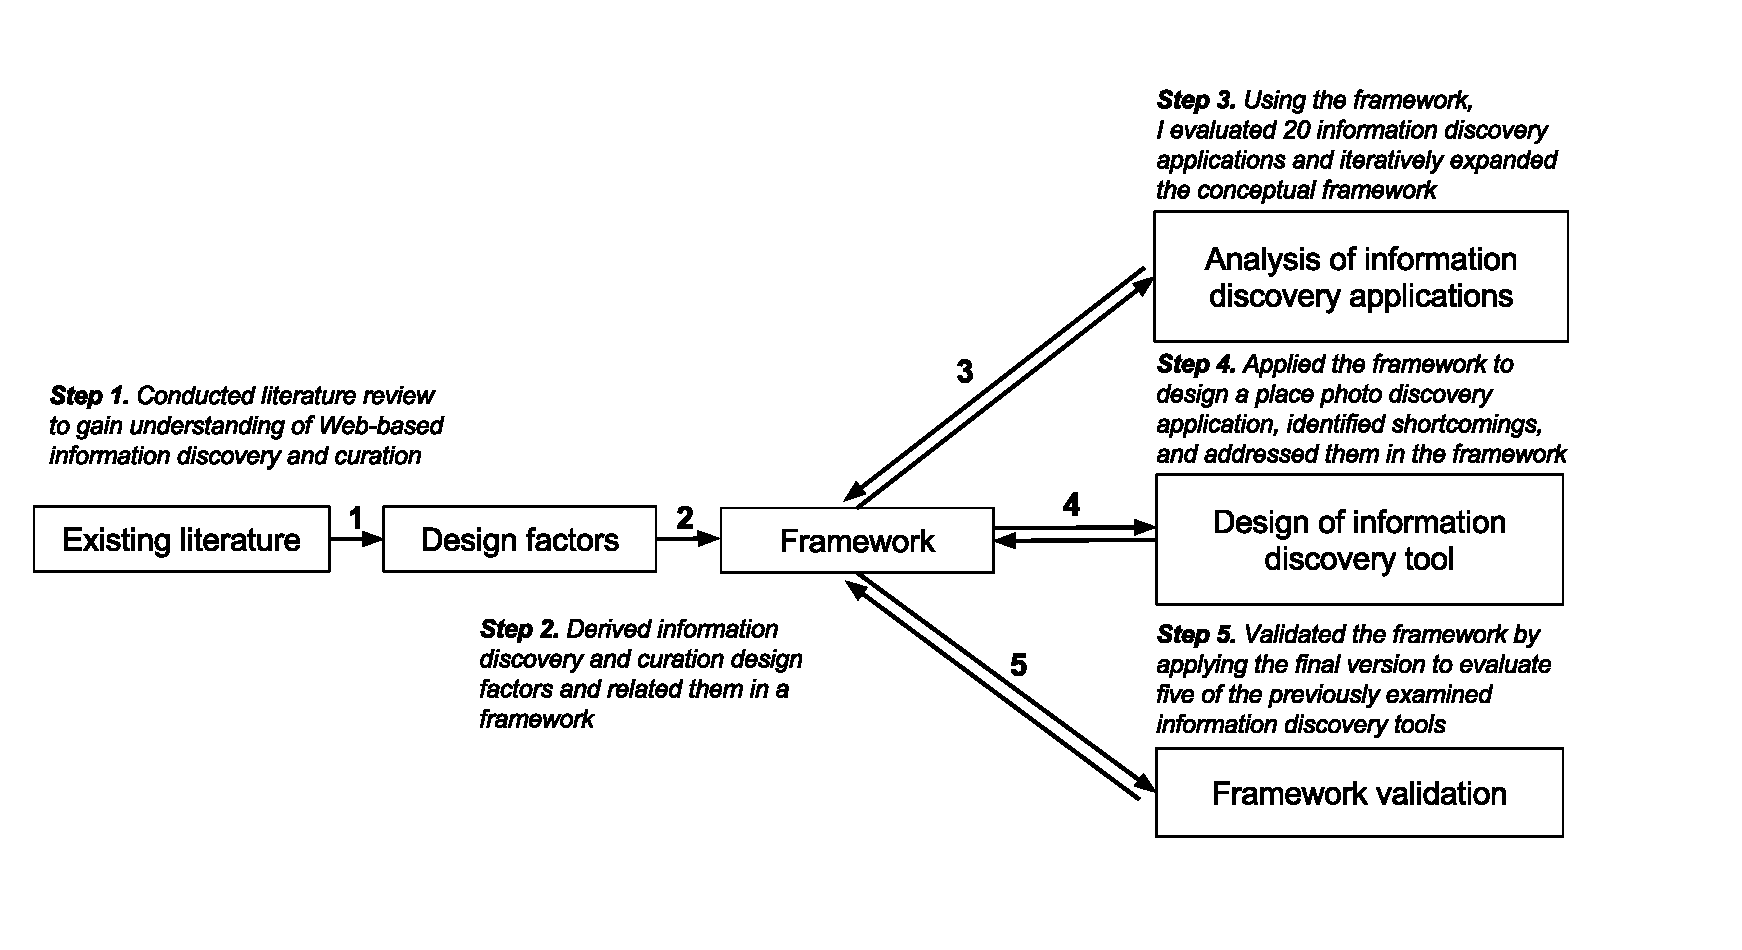
\includegraphics[width=\linewidth]{figures/methodology.pdf}
	\caption{Methodology Overview}
	\label{fig:methodology} 
\end{figure}

{\section{Research Questions and Objective}
This study was designed to address the problem of designing Web applications for information discovery and was motivated by the following research questions and a research objective:

\emph{RQ1:~How do existing Web applications support information discovery?}

\emph{RQ2:~How do existing information discovery applications support information curation?}

\pagebreak 

To address RQ1 and RQ2, I conducted an extensive literature review (see Section~\ref{section:lit_review}) and a case study of 20 information discovery tools (see Section~\ref{section:building}). Using insights from RQ1 and RQ2, I established my main research objective, which is \emph{\textbf{to develop a framework for performing summative and formative evaluation of Web-based information discovery and curation tools}}. I further address my methodology for building the conceptual framework in Sections~\ref{section:building}, \ref{section:applying}, and \ref{section:validating}.

}% end section

{\section{Literature Review}
\label{section:lit_review}
The development of the framework began with an extensive literature review. A diverse set of topics contributed to forming an understanding of information discovery and curation, including information behaviour and information seeking models, high-level Web tasks and modes of Web use, exploration-based models of discovery, and methods of personal and social curation. From this review, the preliminary design factors for the framework were derived. Key findings in the current literature are presented in Chapter~\ref{chapter:chapter_related_work}.
}% end section

{\section{Building and Refining the Conceptual Framework}
\label{section:building}
Through a careful analysis of 20 information discovery applications (see Table~\ref{table:tools}), the framework was iteratively expanded by adding new concepts and establishing relations between those concepts.  The framework was refined as I explored the literature and available tools, and for presentation purposes in this thesis, I present only two versions of the framework. The preliminary framework was a result of this tool analysis and depicted in Chapter~\ref{chapter:old_framework}. The final version of the framework (see Chapter~\ref{chapter:framework}) was a result of developing an information discovery application based on the preliminary work.    

For my case study, I selected some of the most used information discovery applications today and considered the full range of features in those tools (both by referring to the literature and documentation on those tools, as well as exploring the features). The popularity of information discovery applications was determined using Website popularity ranks provided by Alexa\footnote[1]{Alexa is available at www.alexa.com}, a commercial Web traffic data provider. The focus was on applications that had strong information discovery components and lesser priority was given to applications whose purpose revolved only around curation.

I used Yin's strategies for designing a case study~\cite{yin2014case} for guidance. The motivation behind choosing a case study over other methods of qualitative research was based on my choice of research questions, the lack of control over existing applications and their development, and having to focus on contemporary use of real-life Web applications. According to Yin~\cite{yin2014case}, a case study would be an optimal research strategy given the above characteristics.

My study consisted of 20 cases, whereby each case is a Web application that focuses on the support of information discovery. I examined the overall purpose of each application, its description as defined within the application, as well as literature and documentation related to the application (if they were available) against the features that the application provided. For example, if an application provided bookmarking features, I checked if it was indeed intended to be used for information preservation. 

Consequently, the methodology was an iterative process of selecting cases, analyzing them, and determining whether they could be described and evaluated using the framework. If I found a key feature that could not be described, I adapted the framework according to the findings. I repeated the process of case selection and evaluation until the framework was usable for all cases. I then grouped the elements of the framework into categories, recording corresponding questions to ask in order to evaluate applications. 

A list of the tools that were used in this study are presented in Table~\ref{table:tools}. Summaries of their evaluations using the preliminary framework can be found in Appendix~\ref{chapter:appendix_tools}. Other tools were considered throughout the study, however, only the 20 applications presented underwent systematic examination. 

\begin{table*}[htbp]
\small
\caption{Web-based Information Discovery and Curation Tools as of May 15, 2014}
\label{table:tools} 

\begin{tabular}{|p{0.20\linewidth}| p{0.30\linewidth}| p{0.45\linewidth}|}

\hline
\textbf{Application} & \textbf{Address} & \textbf{Description}
\\
\hline
Pinterest       & www.pinterest.com 	& Visual discovery tool \\
\hline
Delicious       & delicious.com 		& Social bookmarking service \\
\hline
Tumblr          & www.tumblr.com 		& Microblogging platform \\
\hline
StumbleUpon     & www.stumbleupon.com  	& Web page discovery tool \\
\hline
Wikipedia       & en.wikipedia.org   	& Free content Internet encyclopedia\\
\hline
Google Maps     & www.google.ca/maps  	& Web mapping service\\
\hline
Rotten Tomatoes & www.rottentomatoes.com & Movie and TV database\\
\hline
500px           & 500px.com            	& Photography site\\
\hline
BucketList      & bucketlist.org  		& Goal tracking and discovery service\\
\hline
We Heart It     & weheartit.com 		& Visual discovery tool \\
\hline
Scoop.it!       & www.scoop.it 			& Online publishing platform \\
\hline
Google Images   & images.google.com  	& Image discovery service \\
\hline
Vimeo           & vimeo.com  			& Video sharing Website\\
\hline
LifeHacker      & lifehacker.com        & Daily blog \\
\hline
YouTube         & www.youtube.com 		& Video hosting platform \\
\hline
Yelp            & www.yelp.ca  			& Business review site\\
\hline
IMDb            & www.imdb.com  		& Movie database \\
\hline
Trip Adviser    & www.tripadvisor.ca 	& Travel site \\
\hline
Urban Spoon     & www.urbanspoon.com    & Online bar and restaurant guide\\
\hline
Thesaurus       & thesaurus.com         & Online thesaurus \\
\hline
\end{tabular}
\end{table*}
} % end section
\pagebreak
{\section{Applying the Framework to the Design of an Information Discovery and Curation Application}
\label{section:applying}

In order to analyze the framework's capabilities when designing for information discovery and curation, I used the framework as a guide for developing a place photo discovery application. The motivation for choosing a place photo discovery application was based on the gaps that were exposed during analysis of some of the applications, such as Google Maps and Pinterest. Applying the framework to designing an application has triggered more changes within the framework, its further extension and refinement. The resulting application is discussed in Chapter~\ref{chapter:application}.
}% end section

{\section{Framework Validation}
\label{section:validating}
In order to further validate the framework, it was applied to the reevaluation of five of the previously examined tools for comparison purposes (see Chapter~\ref{chapter:application}). For each tool, I identified gaps and proposed directions for future development. 
}% end section

{\section{Limitations}
The case study I conducted has a number of limitations. A lack of documentation, research literature, and formal descriptions of available features for some applications introduces a threat to the construct validity of the study. In addition, information discovery tools and features can be used in unintended or unforeseen ways by designers and developers. Therefore, the recorded use of some features within information discovery applications was recorded on my interpretations. To compensate for such limitations, I personally employed the tools over an extended period of time to gain a deeper understanding of their use. In addition, I considered some cases with similar functionality and design to be able to validate or clarify prior findings. 

Many Web applications evolve rapidly. Therefore, my tool analysis only applies to tools at the moment of the study. Additionally, framework validation was performed on five of the previously examined tools, introducing another limitation to the study. 
\pagebreak

Only Web applications running in browsers on a desktop computer were considered in this study. The study can be extended with use of various devices, such as smartphones and tablets, as information discovery patterns and mechanisms may vary for different platforms. 

Another limitation was the lack of prior research on the subject matter. Some researchers have studied information seeking models and high-level Web tasks, but there is a lack of literature on how to enable and support different Web tasks. This opens up opportunities for future research to analyze methods of developing and building frameworks for facilitating and evaluating tools that support other Web tasks, such as communication, transactions, and goal realization.

\section{Conclusion}

\section{Acknowledgments}


% Balancing columns in a ref list is a bit of a pain because you
% either use a hack like flushend or balance, or manually insert
% a column break.  http://www.tex.ac.uk/cgi-bin/texfaq2html?label=balance
% multicols doesn't work because we're already in two-column mode,
% and flushend isn't awesome, so I choose balance.  See this
% for more info: http://cs.brown.edu/system/software/latex/doc/balance.pdf
%
% Note that in a perfect world balance wants to be in the first
% column of the last page.
%
% If balance doesn't work for you, you can remove that and
% hard-code a column break into the bbl file right before you
% submit:
%
% http://stackoverflow.com/questions/2149854/how-to-manually-equalize-columns-
% in-an-ieee-paper-if-using-bibtex
%
% Or, just remove \balance and give up on balancing the last page.
%
\balance{}

% REFERENCES FORMAT
% References must be the same font size as other body text.
\bibliographystyle{SIGCHI-Reference-Format}
\bibliography{refs}

\end{document}

%%% Local Variables:
%%% mode: latex
%%% TeX-master: t
%%% End:
